\documentclass{article}

% imports
\usepackage{xcolor}     % colorize text
\usepackage{graphicx}   % images
\usepackage{hyperref}   % hyperlinks
\usepackage{wrapfig}    % wrapped figures
\usepackage{glossaries} % optional glossary
\usepackage{lipsum}     % easy lorem ipsum
\usepackage{float}      % better image positioning

% overrides & setup
\usepackage[nottoc,numbib]{tocbibind}      % include bibliography in toc
\usepackage[figurename=Abbildung]{caption} % rename Figure to Abbildung
\renewcommand{\refname}{Quellen}
\renewcommand{\contentsname}{Inhaltsverzeichnis}
\graphicspath{{./images/}}
\hypersetup{
    colorlinks=true,
    linkcolor=black,
    citecolor=black,
    filecolor=black,
    urlcolor=black,
}

\begin{document}
    \begin{titlepage}
    \begin{center}
        \Huge
        \textbf{Solarzellen}

        \vspace{0.5cm}

        \LARGE
        Funktion und Stand der Technik bei Stand-Alone-Anlagen

        \vspace{1.5cm}

        \href{mailto:erik.buennig@fh-erfurt.de}{
            \color{black}{
                \textbf{Erik Bünnig}
            }
        }\\
        18.2.2021

        \vfill

        \Large
        Projektarbeit zur alternativen Prüfungsleistung im Kurs Elektrotechnik

        \vspace{1.5cm}

        \href{https://www.fh-erfurt.de/fhe/}{
            
\includegraphics[scale=0.5]{fhe_logo}
        }
    \end{center}
\end{titlepage}

    \tableofcontents
    \thispagestyle{empty}
    \newpage

    \pagenumbering{arabic}

    \section{Vorwort}
    Diese Facharbeit dient als alternative Prüfungsleistung für den
Kurs Elektrotechnik (Angewandte Informatik, B.Sc.) an der
Fachhochschule Erfurt und behandelt photovoltaische Zellen, deren
Anwendungsgebeite und Funktionsweise sowie einen Teil der
Historie der Photovoltaik.
\\\\
Für lesen der digitalen Kopie dieser Facharbeit: alle
Quallenangaben sind mit \textit{hyperlinks} verlinkt, Referenzen
führen direkt per \textit{hyperref} zu der dazugehöhrigen Quelle.
Alle Sektionen können vom Inhaltsverzeichnis per klick erreicht
werden.
\\\\
Diese Arbeit wurde mit \LaTeX{} erstellt, Source Code ist verfügbar unter:
\begin{center}
    \hyperlink{https://github.com/erxkk/projektarbeit-elektrotechnik}
    {github/erxkk/projektarbeit-elektrotechnik}
\end{center}
    \newpage

    \section{Einleitung}
    \subsection{Begrifflichkeiten}
    \subsubsection{Photoelektrischer Effekt}
        Wechselwirkung zwischen Photonen und baryonischer Materie,
        wird in den inneren und äußeren photovoelektrischen Effekt
        und die Photoionisation unterteilt. Beschreibt die Freisetzung
        von Elektronen durch Bestrahlung eines Materials mit
        elektromagnetischer Strahlung \cite{Wiki_PhotoelectricEffect}.

    \subsubsection{Photovoltaischer Effekt}
        Teil des inneren photoelektrischen Effekts, beschreibt Bildung
        eines Photostroms entgegen der Durchlassrichtung des p-n-Übergungs
        als Folge von elektromagnetischer Bestrahlung. Dabei werden
        Ladungsträgerpaare in den dotierten Schichten der des Materials
        getrennt, daworaufhin sich Elektronen in den n-dotierten
        Schichten und die Löcher in den p-dotierten Schichten ablagern
        in so fern sie auf dem weg dahin nicht mit entgegen gesetzen
        Ladungsträgern zusammenstoßen. Der photovolatische Effekt baut
        auf der Photoleitung auf, einem weiterm inneren Teil des
        photoelektrischen Effekts. Der photovoltaische Effekt dient
        als Grundlage für die Funktionsweise von photovoltaischen Zellen
        \cite{Wiki_PhotoelectricEffect}.

    \subsubsection{Photovoltaische Zelle}
        Elektrisches Bauelement das auf Grundlage des photvoltaischen
        Effekts, Strom erzeugt und vorwiegend aus Silizium oder anderen
        Halbleitermaterialien besteht.\\
        Umgangssprachlich werden photovoltaische Zellen oft Solarzellen
        genannt, dabei wird der Begriff auch als Synonym für Solarpanäle
        benutzt obwohl diese eine Ansammlung von photolotaischen Zellen,
        Leiterelementen und strukturellen Bauelementen beschreiben.

\newpage

\subsection{Historie der Photovoltaik}
    \subsubsection{Entdeckung}
        Die Effekte der Photovoltaik wurden erstmals in 1839 von Andre
        Edmond Becquerel entdeckt, aber erst weit später praktisch
        angewendet. Bei der Entdeckung handelte es sich um einen geringen
        Strom zwischen einer Platin-Anode und -Kathode welcher sich unter
        Licht verstärkte. \cite{Wiki_PhotovoltaicHistory}

    \subsubsection{Nennenswerte Ereignisse}
        \begin{itemize}
            \item 1876 - Beweis der direkten Konversion von
                elektromagnetischer Strahlung in elektrische Energie durch
                William Grylls Adams und Richard Evans Day
            \item 1907 - Theoretische Erklärung des photoelektrischen Effekts
                auf Basis der Lichtquantenhypothese (1905) durch Albert
                Einstein
            \item 1912 - 1916 - Experimentelle Bestätigung von Einsteins
                Erklärung durch Robert Andrews Millikan
            \item 1958 - Erste Verwendung von Solarzellen zur Versorgung
                eines Satelliten der NASA (Vanguard I) \cite{Wiki_Vanguard}
        \end{itemize}
    \newpage

    \section{Grundlegender Aufbau und Funktionsweise}
    \subsection{Aufbau}
    Die meisten photovoltaischen Zellen haben den gleichen Grundaufbau
    und nur geringe Unterscheide wie das Muster der vorderen Kontakte
    oder die chemische Komposition der Anti-Reflexionschicht.
    \begin{figure}[H]
        \centering
        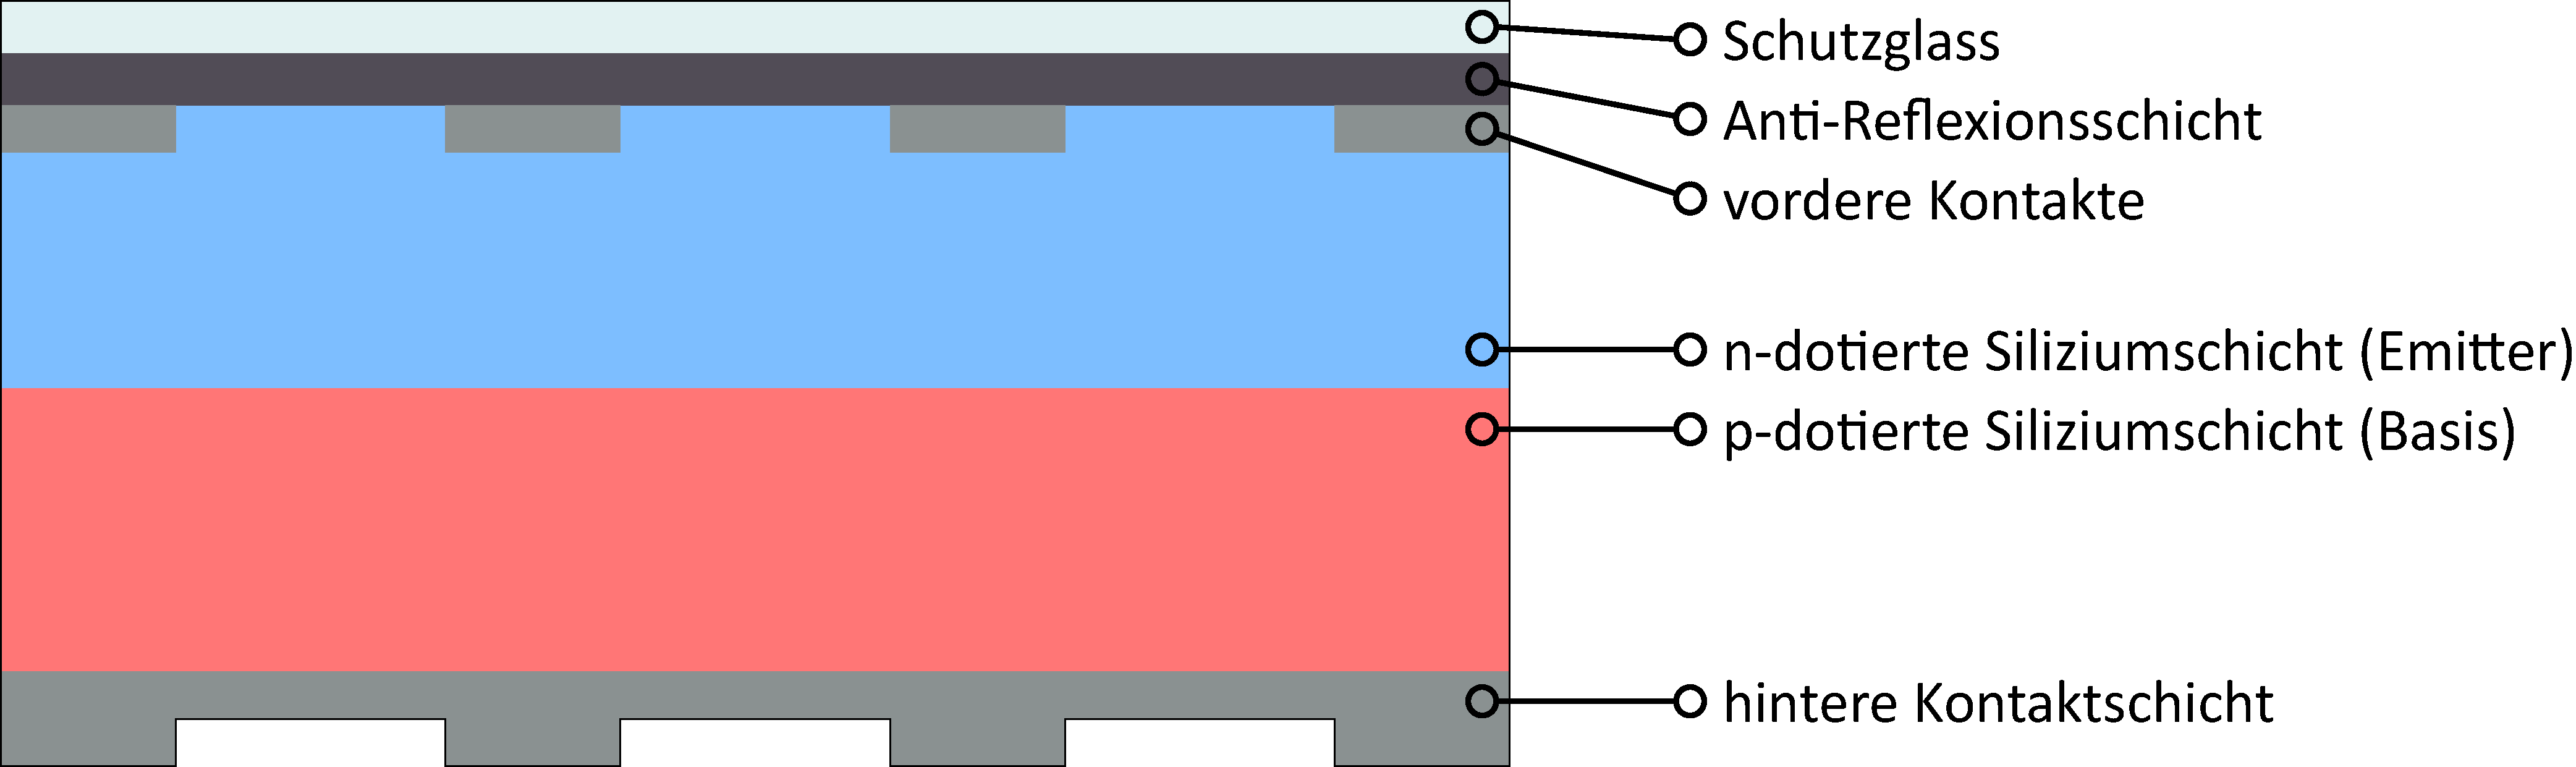
\includegraphics[width=1.0\linewidth]{solarzelle_schnitt.pdf}
        \caption{Grunlegender Aufbau einer Silizium-basierten Solarzelle}
    \end{figure}
    Die Dotierung der Schichten beschreibt einen Prozess bei dem ein
    Siliziumkristall mit Unreinheiten besetzt wird um dessen elektrische
    Leitfähigkeit zu beeinflussen. Silizium hat 4 Valenzelektronen und
    bildet somit Kristallstrukturen durch Kovalente Bindungen. Durch
    das dotieren mit Atomen mit mehr als 4 Valenzelektronen entsteht
    eine n-dotierte Schicht, bei dotieren mit Atomen mit weniger als 4
    Valenzelektronen eine p-dotierte Schicht.

\subsection{Funktionsweise}
    Wenn eine Solarzelle von Licht mit einer Wellenlängen von maximal
    1110nm getroffen wird welche nicht reflektiert werden, können diese
    bei Interaktion mit Atomen in den p- und n-dotierten Schichten
    Elektronen-Loch-Paare erzeugen.
    \begin{figure}[H]
        \centering
        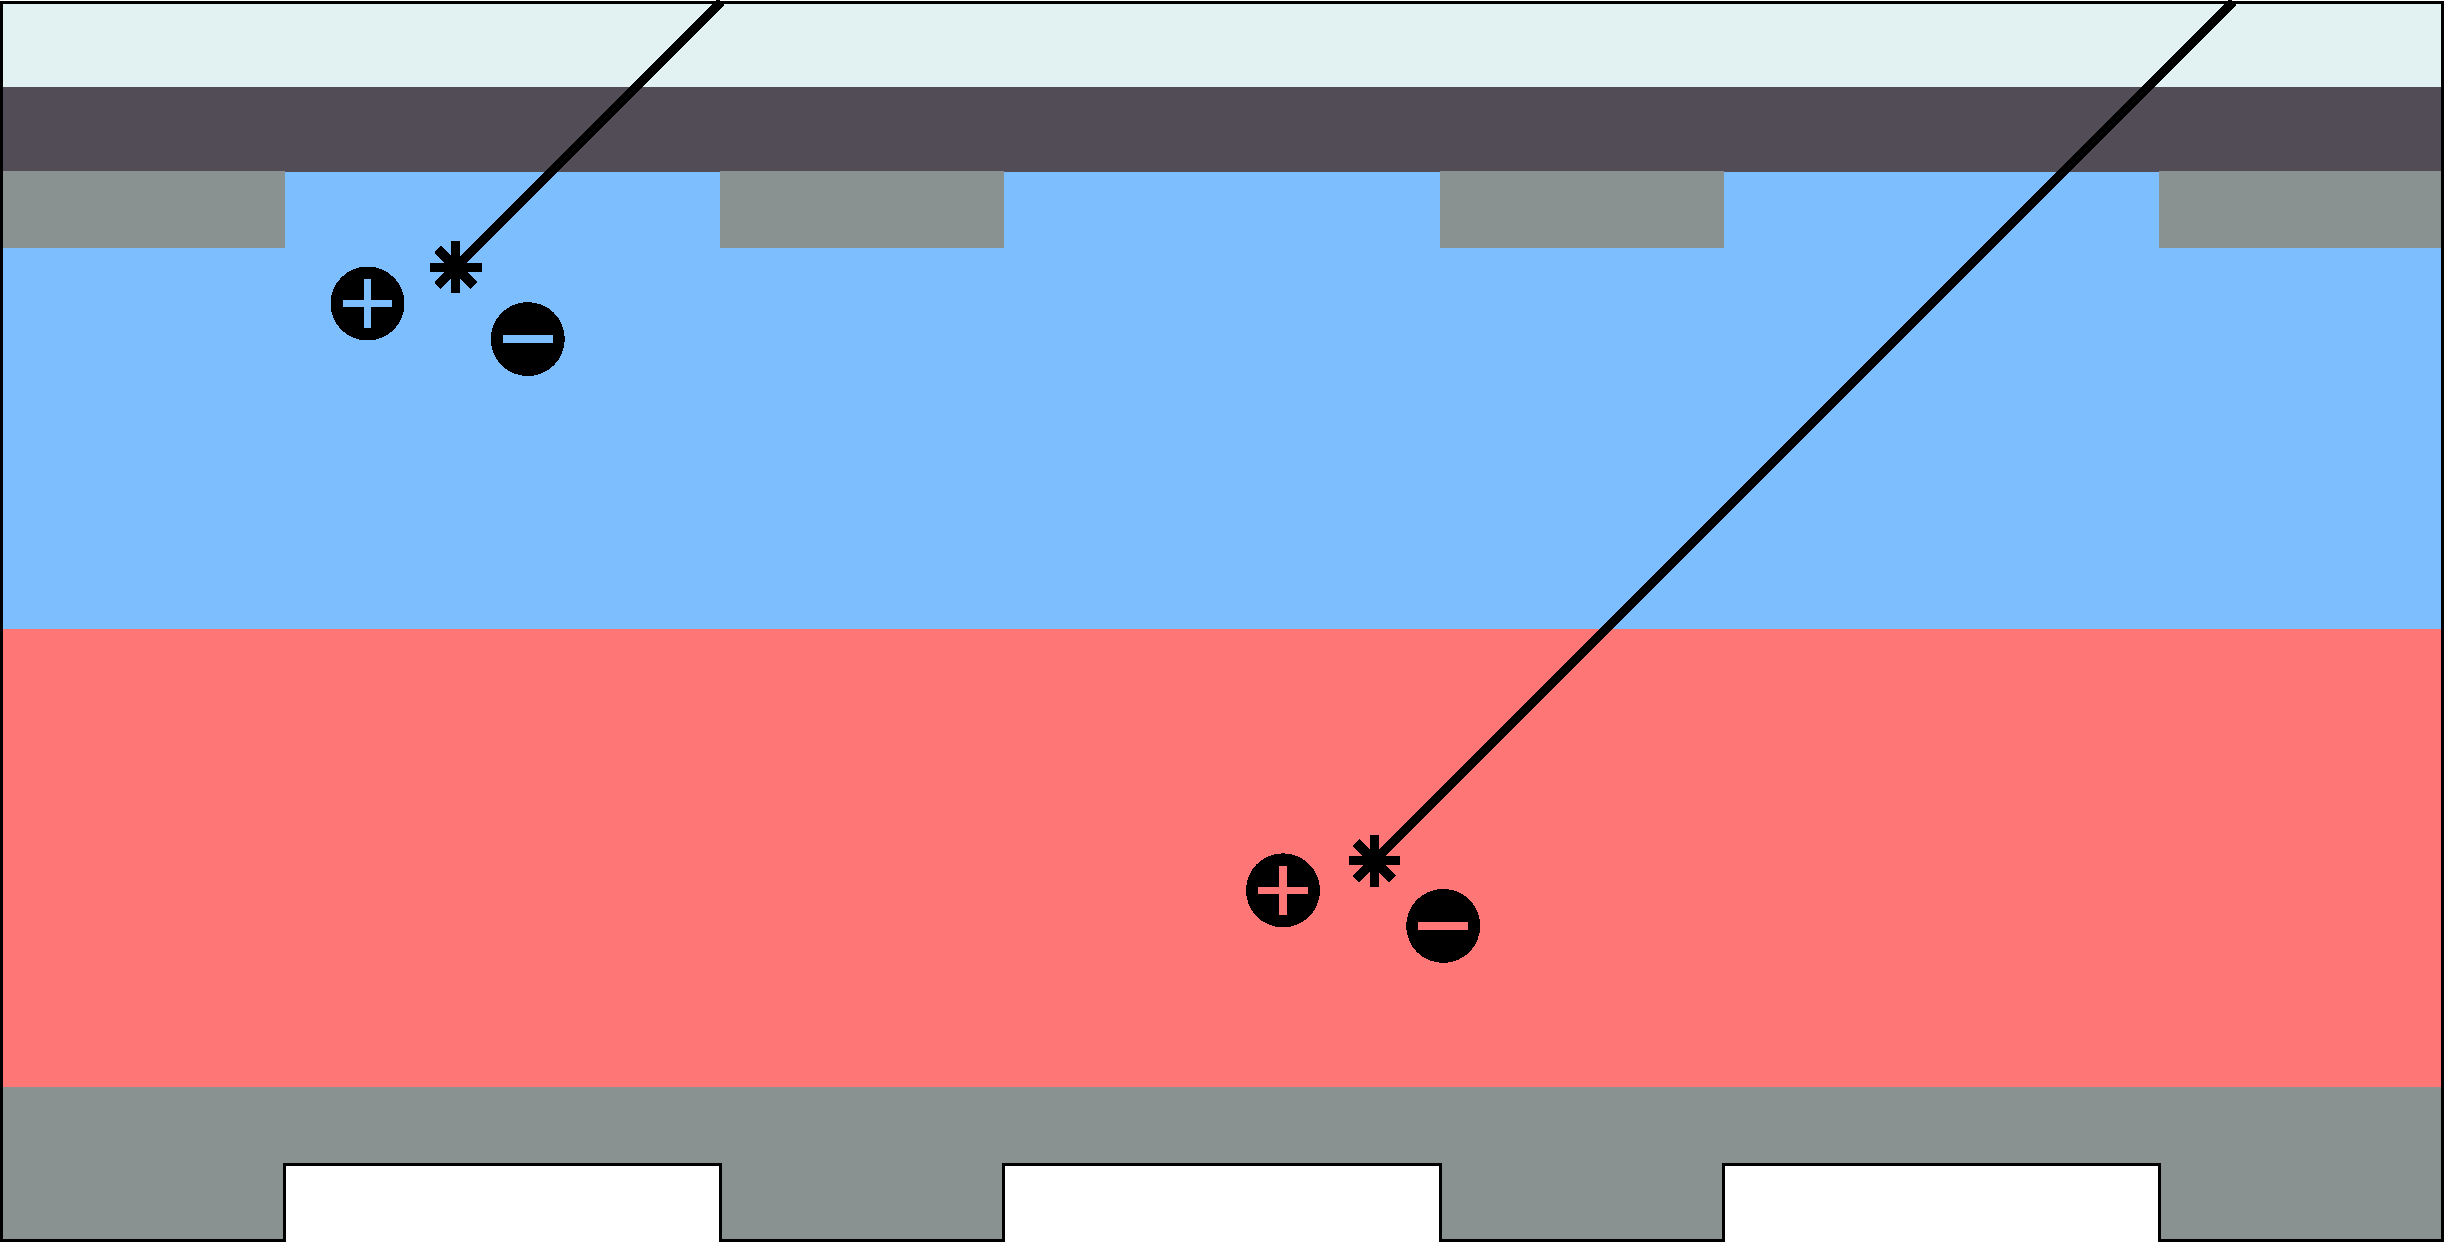
\includegraphics[width=0.65\linewidth]
        {solarzelle_schnitt_schritt1.pdf}
        \caption{Bildung von Elektronen-Loch-Paaren}
    \end{figure}

\newpage

    Durch den photovoltaischen Effekt bewegen sich die befreiten
    Elektronen in Richtung der der n-dotierten Schicht (blau) und
    Löcher in Richtung der p-dotierten Schicht (rot).
    \begin{figure}[H]
        \centering
        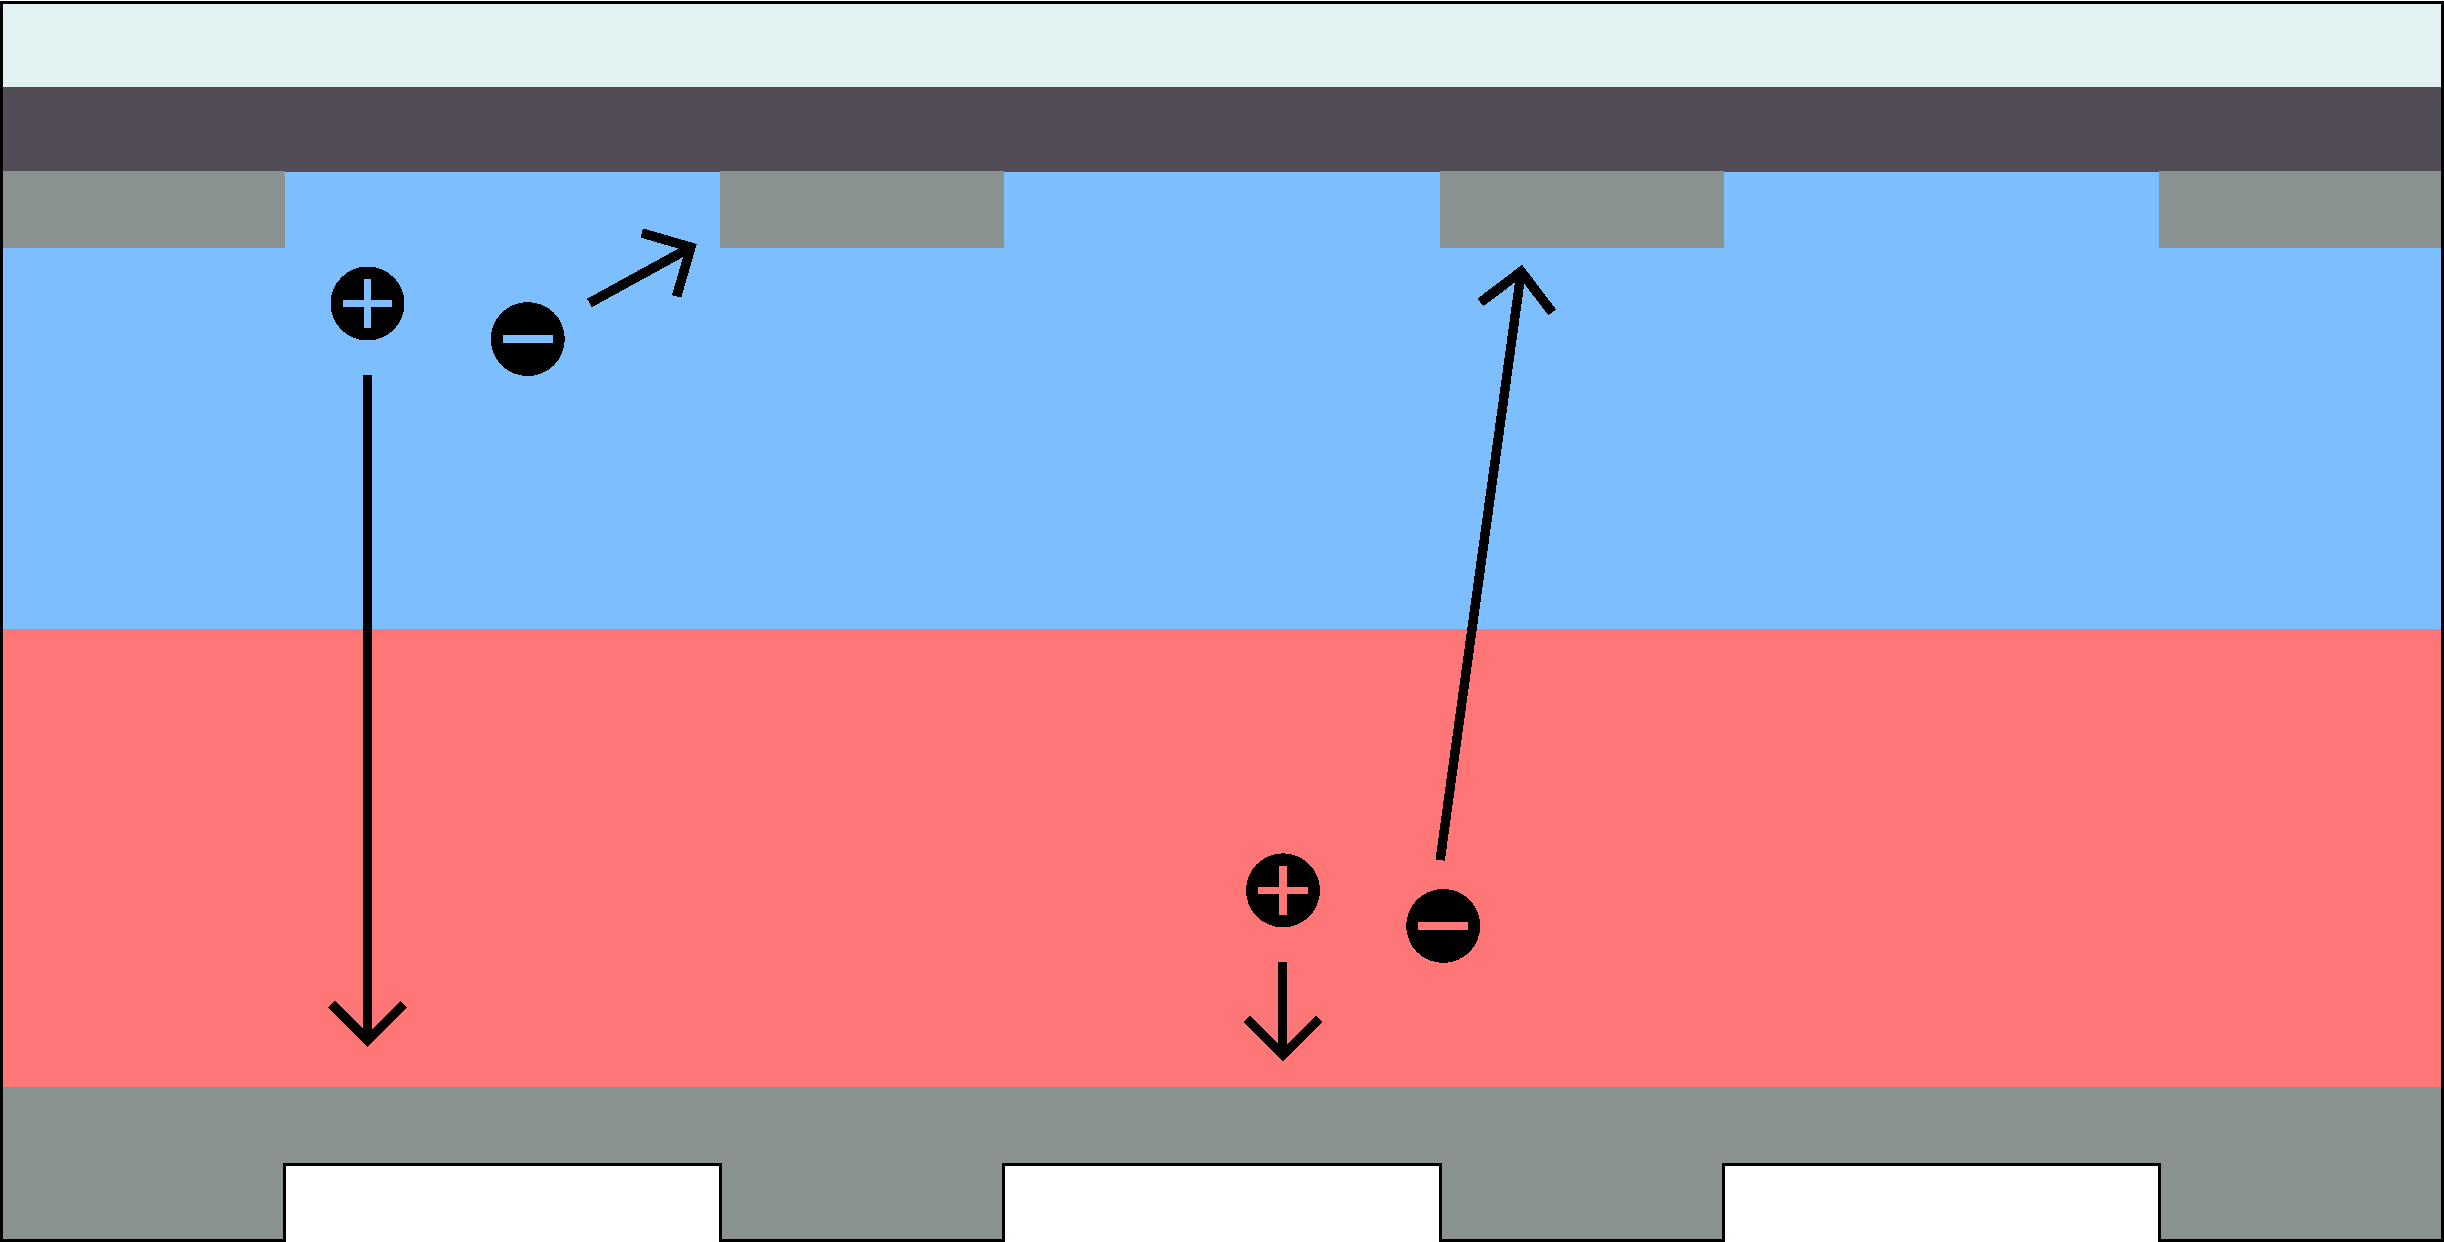
\includegraphics[width=0.65\linewidth]
        {solarzelle_schnitt_schritt2.pdf}
        \caption{Bildung des Photostroms}
    \end{figure}
    Der dabei entstehende Strom nennt sich Photostrom und die dabei
    Entstehende Potentialdifferenz erzeugt eine Spannung welche bei
    Anlegen eines externen Verbrauchers an die oberen und unteren
    Kontakte einen Messbaren Strom erzeugt.
    \begin{figure}[H]
        \centering
        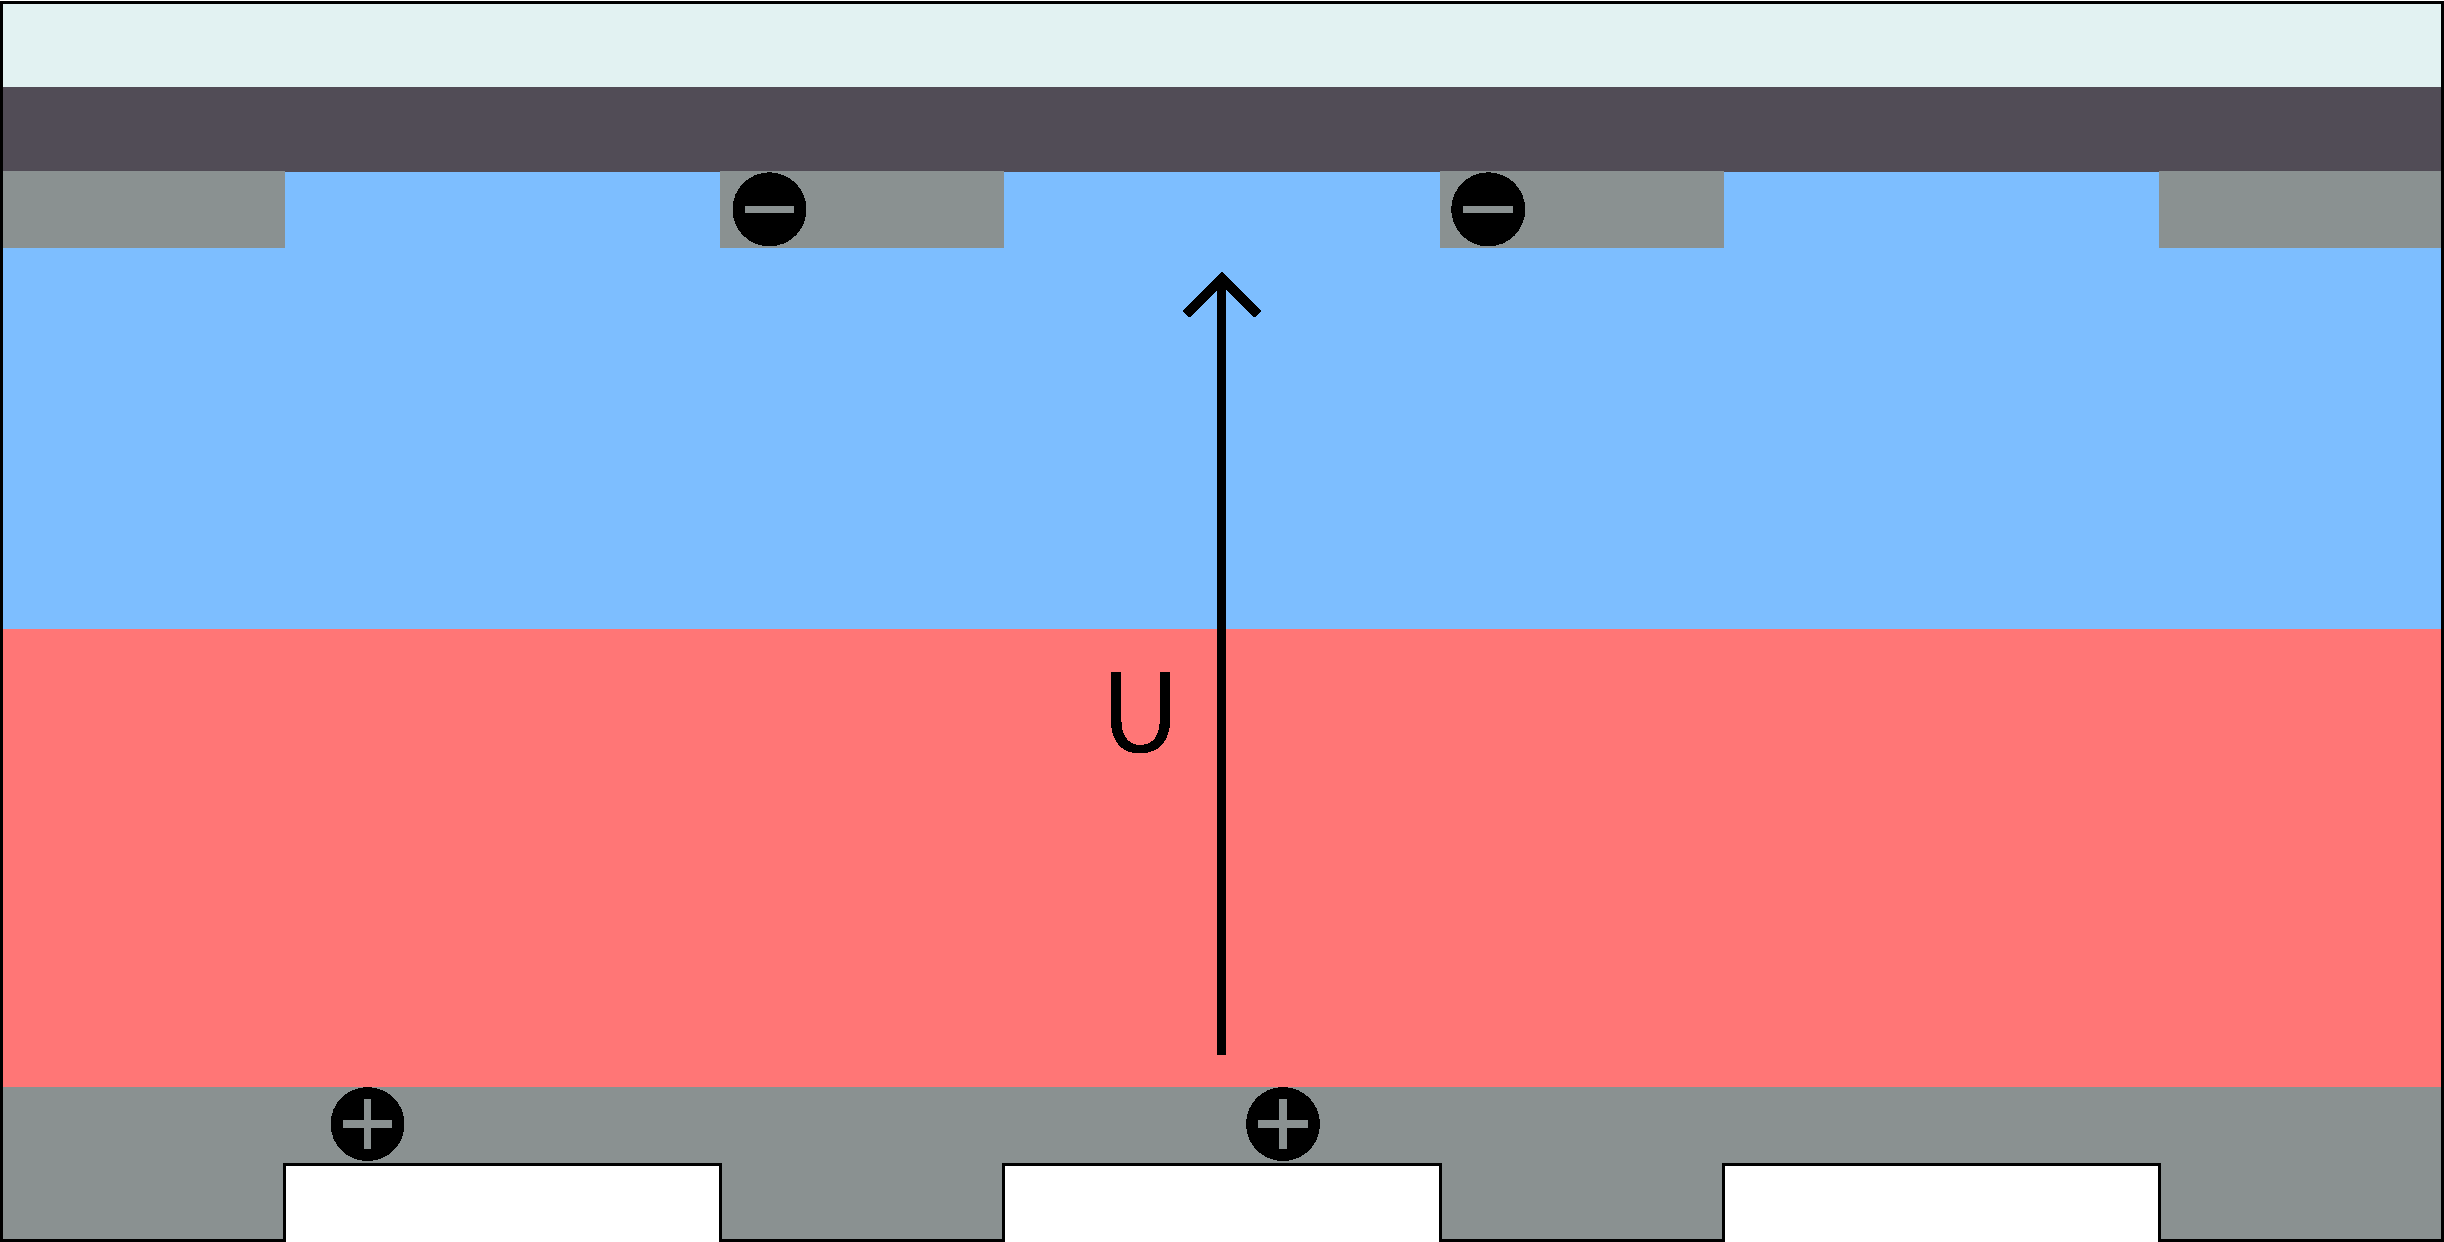
\includegraphics[width=0.65\linewidth]
        {solarzelle_schnitt_schritt3.pdf}
        \caption{Entstehen einer messbaren Spannung}
    \end{figure}
    Erst wenn ein externer Verbraucher angeschlossen ist, bewegen
    sich Elektronen und Löcher zu den nahe gelegenen Kontakten und
    dann über den Verbraucher zurück in die jeweiligen Sichten.

\subsection{Vorteile}
    Nach der Installation von Solarzellen ist kein Rohmaterial oder
    Energiezufluss benötigt um Energie zu sammeln. Dadurch das
    Solarzellen keine beweglichen oder kontaktintensiven Teile besitzen
    brauchen sie beinahe keine Wartung und sind unanfällig gegenüber
    feuchten Witterungsverhältnissen \cite{SolarMaintenance}.\\
    Auch wenn Solarzellen wegen ihrer Umweltunfreundlichen Herstellung
    oft kritisiert werden, ist der Erntefaktor \footnote{Beschreibt das
    Verhältnis zwischen Erzeughter zu verbrauchter Energie} von
    Solarzellen etwa 26:1 (4\% Energieoffset) im vergleich zu den
    durchschnittlich 9:1 (11\% Energieoffset) von Kohle- und
    Ölkraftwerken \cite{SolarCarbonEmissions}.

\subsection{Nachteile}
    Solarzellen sind Anfällig für Temperaturschwankungen, bei
    höheren Temperaturen sinkt die Effizienz von Solarzellen. Die
    durschnittliche Energieeffizienz von Solarzellen liegt bei etwa
    15\% bis 20\% (unter Laborkonditionen) \cite{SolarEfficiency}, das
    heißt das rund 85\% bis 80\% der aufgefangenen Sonnenenergie
    entweder reflektiert oder in Wärme umgewandelt wird welche wiederum
    die Effizienz verringert (die überflüssige thermische Energie kann
    allerdings zur Effizienzsteigferung beitragen indem sie zur
    Versorgung von Kühlungsanlagen verwendet wird.
    \cite{YouTube_RE-SolarFlaw, PhotovoltaicPrinciples} Chapter 3,
    Page 22/24).\\
    Solarzellen können nur am Tag Energie produzieren und ihre Effizienz
    sinkt in den Herbst- und Wintermonaten. Photovoltaische Zellen bieten
    nur dann eine ernstzunehmende Alternative für Nuklear-, Wind-, Hydro-
    oder sogar fossile Energie wenn die aufgesammelte Energie auch
    effizient gespeichert und transportiert werden kann.
    \newpage

    \section{Anwendungsgebiete}
    \subsection{Niedrigverbrauchapplikationen}
    Solarzellen eignen sich hervorragend zur Energieversorgung für
    vorwiegend bedienungsfreie Applikationen wie eigenständige
    Sensoren (z.B.: Wetterstation, Luft- oder Wasserqualitätssensoren),
    da diese oft einen geringen stetigen Energieverbrauch aufweisen,
    welcher bei Nacht oder schlechten Wetterverhältnissen mit einer
    Batterie überbrückt werden kann.

\subsection{Raumfahrt}
    Auch für die Stromversorgung von Satelliten oder Raumstationen
    eignen siche Solarzellen hervorragend, da im Vakuum das Auffangen
    elektromagnetischer Strahlung nicht durch atmosphärische Effekte
    beeinflusst wird. Die geringe Masse der Zellen und die draus
    resultierenede Treibstoffeffizienz ist ein weiterer Grund für die
    Nutzung in der Raumfahrt.

\subsection{Alternative zu fossilen Brennstoffen}
    \subsubsection{Kalifornien, USA}
        Der US-Bundesstaat Kalifornien beitet ein gutes Besipiel für
        sowohl Vorteile als auch Nachteile von Solarenergie. In
        hinreichend sonnigen Regionen wie Kalifornien reicht die
        durschnittliche durch Solar produzierte Energie zum Decken des
        durschnittlichen Energieverbrauchs aus. Allerdings sind sowohl
        Produktion als auch Verbrauch von Energie nicht konstant.
        Solaranlagen produzieren ihre Energie hauptsächlich zwischen
        7 Uhr und 18 Uhr.
        \begin{figure}[H]
            \centering
            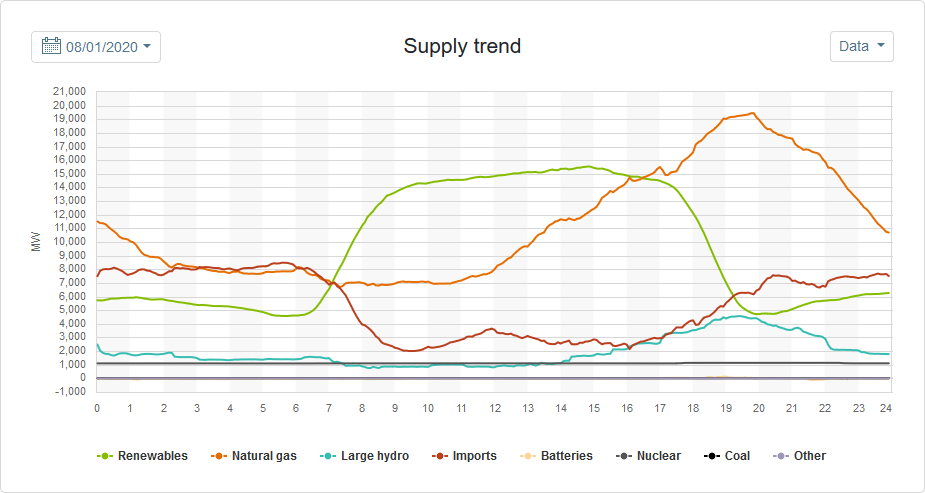
\includegraphics[width=0.9\linewidth]
            {california_supply_2020-08-01.png}
            \caption{Angebot an Energie in Kalifornien, USA, 01.08.2020
                \cite{Img_CaliforniaSupply}
            }
        \end{figure}
        Der tägliche Verbrauch erreicht vorallem um 17 Uhr bis 22 Uhr
        Höchstwerte. Nächte und Schlechtwettertage müssen dann durch
        gespeicherte, importierte oder lokale nicht-Solarenergie überbrückt
        werden, trotz der großartigen Vorraussetzungen für Solarenergie.
        \cite{SolarCalifornia, YouTube_RE-California}
        \begin{figure}[H]
            \centering
            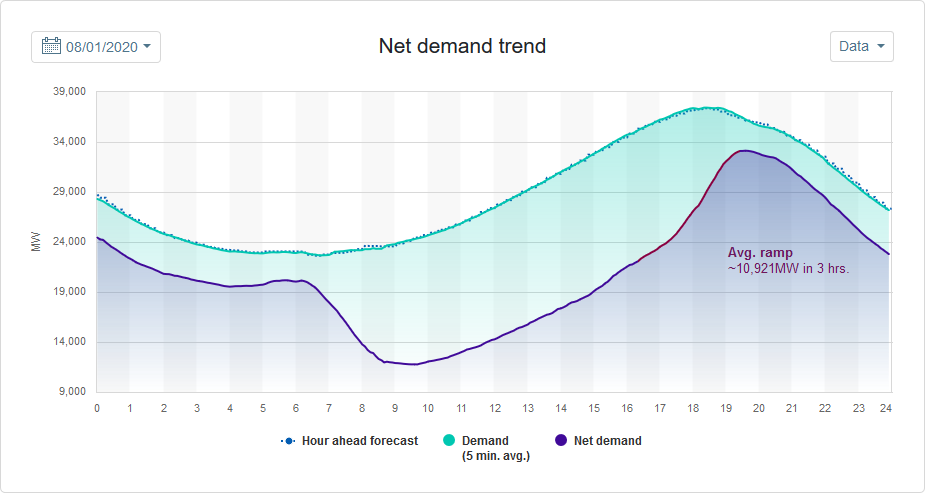
\includegraphics[width=0.9\linewidth]
            {california_demand_2020-08-01.png}
            \caption{Nachfrage an Energie in Kalifornien, USA, 01.08.2020
                \cite{Img_CaliforniaDemand}
            }
        \end{figure}

    \subsubsection{Deutschland}
        In Deutschland wird Solarenergie seit 2000 zunehmend ausgebaut
        und staatlich gefördert, von 2000 bis 2011 stieg der
        Solarenergieanteil von 64GWh auf 19TWh, befindet sich aber mit
        einem Energienteil von gerade mal rund 7\% (stand 2019) noch
        lange nicht auf dem Niveau von Kalifornien
        \cite{Wiki_PhotovoltaicGermany}.
        \begin{figure}[H]
            \centering
            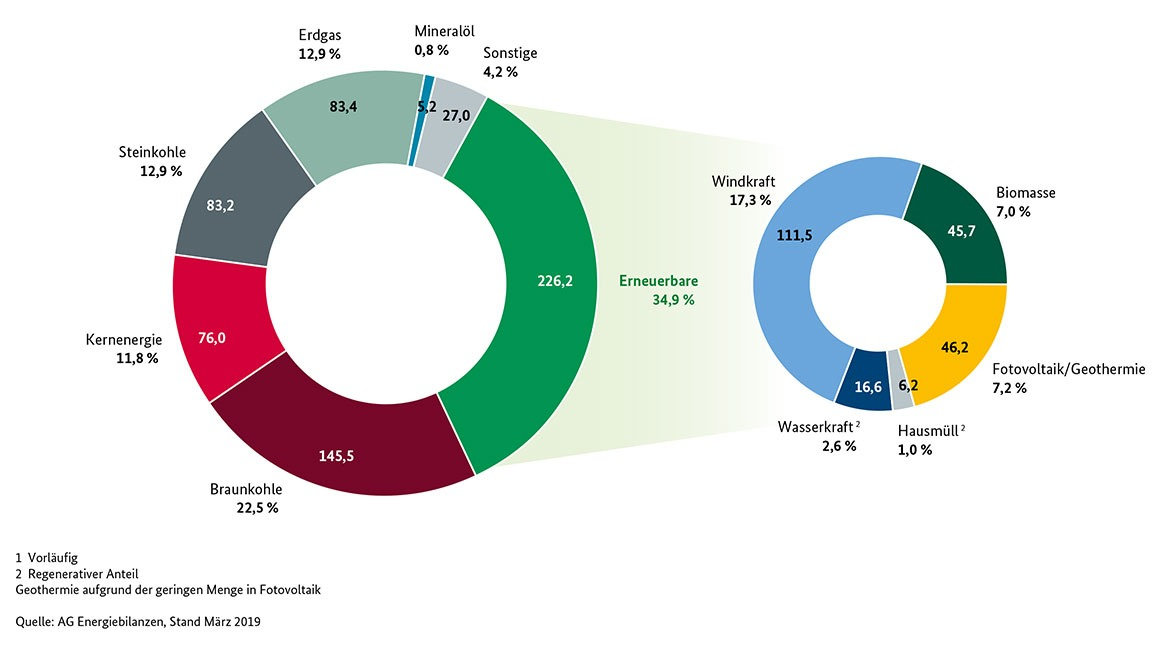
\includegraphics[width=0.9\linewidth]
            {bruttostromerzeugung-in-deutschland.jpg}
            \caption{Anteil der Energieproudktion Deutschland, Stand März
                2019 \cite{Img_GermanySupply}
            }
        \end{figure}
    \newpage

    \section{Anwendungsbeispiel}
    % IoT-Sensor 1..2W betrieb durch solarzelle
% solar zellentyp, größe, kapazität, dunkelheits überbrückung
\subsection{Problemstellung}
    Gegeben sei eine Wetterstation in einem abgelegenen Teil der Sahara,
    welche eine Leistungsaufnahme zwischen 1W und 2W besitzt. Wie kann
    eine solche Anlage kostengünstig und relativ wartungsfrei betrieben
    werden?
\subsection{Entwurf}
\subsection{Konklusion}
    \newpage

    \section{Zusammenfassung}
    \newpage

    \newpage
\begin{thebibliography}{9}
    % Articles
    \bibitem{Wiki_SolarCell}
        \href{https://de.wikipedia.org/wiki/Solarzelle}{
            Wikipedia: Solarzelle
        }\\
        \href{https://en.wikipedia.org/wiki/Solar_cell}{
            Wikipedia: Solarcell (Englisch)
        }

    \bibitem{Wiki_PhotoelectricEffect}
        \href{https://de.wikipedia.org/wiki/Photoelektrischer_Effekt}{
            Wikipedia: Photoelektrischer Effekt
        }

    \bibitem{Wiki_PhotovoltaicHistory}
        \href{https://de.wikipedia.org/wiki/Geschichte_der_Photovoltaik}{
            Wikipedia: Geschichte der Photovoltaik
        }

    \bibitem{Wiki_Vanguard}
        \href{https://de.wikipedia.org/wiki/Vanguard-Projekt}{
            Wikipedia: Vanguard-Projekt
        }

    % Images
    \bibitem{Wiki_Img_PhotodiodeSymbol}
        \href{https://de.wikipedia.org/wiki/Datei:Symbol_Photodiode.svg}{
            Wikipedia: Symbol einer Photodiode
        }

    % Vidoes
    \bibitem{Wiki_Video_RE-SolarFlaw}
        \href{https://www.youtube.com/watch?v=yVOnHWnLSeU}{
            YouTube: Real Engineering - The Mystery Flaw of Solar Panels
        }

    \bibitem{Wiki_Video_RE-California}
        \href{https://www.youtube.com/watch?v=h5cm7HOAqZY}{
            YouTube: Real Engineering - California's Renewable Energy Problem
        }
\end{thebibliography}
\end{document}